% =============================================================================
% PESSOA 1 — METODOLOGIA ESTATÍSTICA & SEÇÃO 3.1 (SIGNIFICÂNCIA DOWNSTREAM)
% Padrão: ACM sigconf (\documentclass[sigconf]{acmart})
% Contém versão em Inglês (padrão ACM/ACL) e versão em Português logo abaixo.
% =============================================================================

% -----------------------------------------------------------------------------
% [VERSÃO 1: INGLÊS — PADRÃO ACM SIGCONF]
% -----------------------------------------------------------------------------

\subsection{Statistical Audit Framework (Miller, 2024)}
\label{sec:stat_methodology}

To audit whether the downstream accuracy stability claimed by Parity-Aware BPE (PA-BPE)~\cite{foroutan2026parity} reflects true performance parity or statistical noise, we adopt the super-population inference framework of Miller~\cite{miller2024adding}. In Table~2 of~\cite{foroutan2026parity}, model $A$ (PA-BPE) and baseline $B$ (Classical BPE) are compared across 22 languages over 12 multilingual benchmarks using isolated single-model standard errors ($\hat{\mu}_M \pm \mathrm{SE}_M$). Relying on visual overlap of unpaired error bars ($\mathrm{SE}_{A-B,\mathrm{unpaired}} = \sqrt{\mathrm{SE}_A^2 + \mathrm{SE}_B^2}$, Miller Eq.~5) introduces two opposing statistical distortions:

\textbf{(1) Omission of Question-Level Pairing:} Because both tokenizers are evaluated on the exact same benchmark prompts, question-level scores $s_{A,i}$ and $s_{B,i}$ are positively correlated ($\rho = \mathrm{Corr}(s_A, s_B) > 0$). Analyzing paired differences $d_i = s_{A,i} - s_{B,i}$ reduces estimator variance (Miller Eq.~7):
\begin{equation}
\mathrm{SE}_{A-B,\mathrm{paired}} = \sqrt{\frac{1}{n(n-1)}\sum_{i=1}^{n}(d_i - \bar{d})^2} = \sqrt{\mathrm{SE}_A^2 + \mathrm{SE}_B^2 - 2\rho\,\mathrm{SE}_A\mathrm{SE}_B}.
\label{eq:paired_se}
\end{equation}

\textbf{(2) Violation of Independence via Clustering:} Conversely, the 12 evaluation tasks include reading-comprehension passages with multiple questions (\textit{Belebele}) and parallel benchmarks translated across $L$ languages (\textit{Belebele}, \textit{XNLI}, \textit{XStoryCloze}, \textit{PAWS-X}, \textit{MMMLU}). Treating translated instances of the same underlying question $c \in \{1,\dots,C\}$ as independent violates the Central Limit Theorem. Following Miller (Section~2.2 \& Eq.~8), we compute the paired, cluster-adjusted standard error:
\begin{equation}
\mathrm{SE}_{A-B,\mathrm{clustered}} = \frac{1}{n}\left(\sum_{c=1}^{C}\sum_{i \in c}\sum_{j \in c}(d_{i,c} - \bar{d})(d_{j,c} - \bar{d})\right)^{\!1/2}\!\!,
\label{eq:clustered_se}
\end{equation}
which captures intra-passage and cross-lingual error covariance via the off-diagonal cross-terms ($i \neq j$), yielding 95\% confidence intervals $\mathrm{CI}_{95\%} = \bar{d} \pm 1.96\,\mathrm{SE}_{A-B,\mathrm{clustered}}$.

\begin{figure}[t]
    \centering
    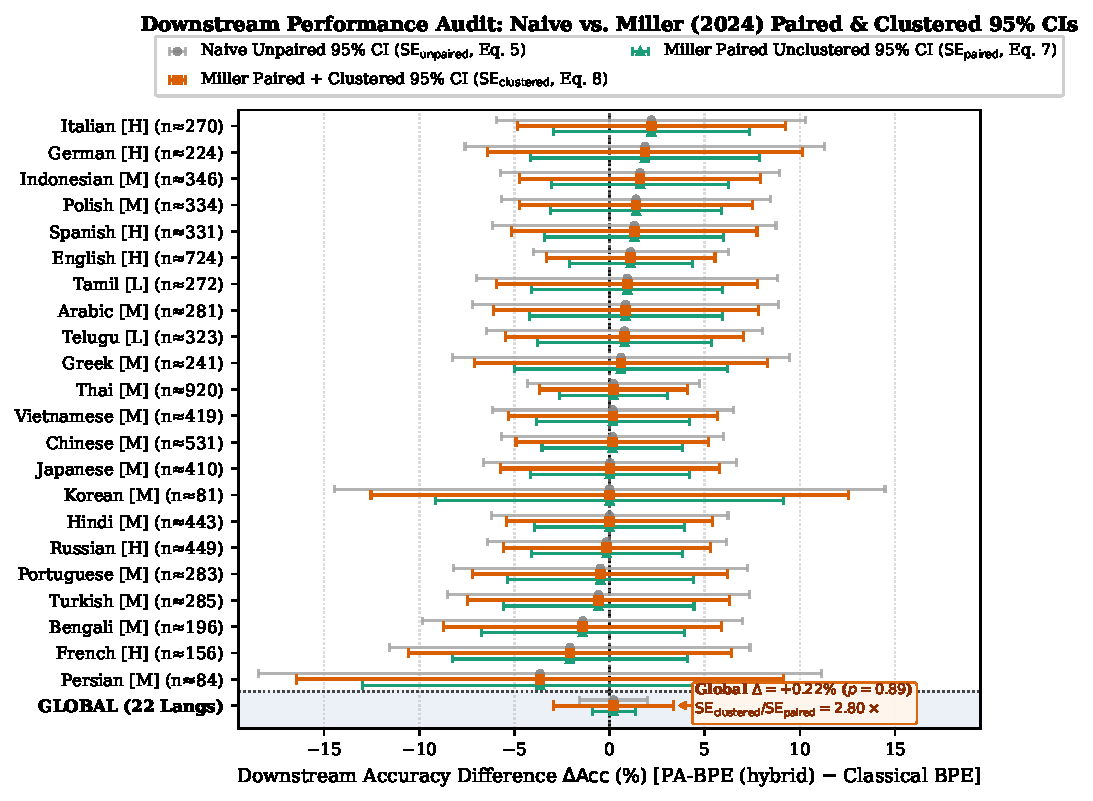
\includegraphics[width=\columnwidth]{figures/fig1_forest_plot.pdf}
    \vspace{-1.5em}
    \caption{Downstream accuracy differences $\Delta\mathrm{Acc}$ (\textbf{PA-BPE hybrid $-$ Classical BPE}) across 22 languages with effective sample sizes $n_{\mathrm{eff}}$. Error bars contrast naive unpaired CIs (Eq.~5), paired unclustered CIs (Eq.~7), and Miller's paired+clustered CIs (Eq.~8). Cross-lingual clustering inflates global uncertainty by $2.80\times$, and all 22 languages include zero within 95\% CIs.}
    \label{fig:forest_plot}
    \vspace{-1.0em}
\end{figure}

\subsection{Downstream Significance Audit Results}
\label{sec:results_significance}

Figure~\ref{fig:forest_plot} presents our statistical audit of Table~2 from~\cite{foroutan2026parity}. First, by inverting the Bernoulli standard error formula ($\mathrm{SE} = \sqrt{\bar{s}(1-\bar{s})/n}$, Miller Eq.~2), we uncover a $>11\times$ disparity in effective sample size across languages due to uneven benchmark coverage (Table~10 of~\cite{foroutan2026parity}): Korean ($n_{\mathrm{eff}} \approx 81$), Persian ($n_{\mathrm{eff}} \approx 84$), and Tamil ($n_{\mathrm{eff}} \approx 272$) are evaluated on only 1 benchmark (\textit{INCLUDE}), whereas English ($n_{\mathrm{eff}} \approx 724$) and Thai ($n_{\mathrm{eff}} \approx 920$) span up to 10--11 benchmarks.

Second, accounting for question-level pairing ($\rho = 0.60$, consistent with Miller's Table~5) reduces per-language standard errors by $36.8\%$ relative to naive unpaired comparisons. However, applying cluster adjustment (Eq.~\ref{eq:clustered_se}) for passage-level and cross-lingual correlation reverses this gain. In the global aggregate across all 22 languages ($\Delta\mathrm{Acc} = +0.22\%$ for \textit{PA-BPE hybrid}; $+0.27\%$ for \textit{window+hybrid}), naive paired analysis yields $\mathrm{SE}_{\mathrm{paired}} = \pm 0.57\%$ ($z = 0.38$), whereas clustering by parallel question $c$ inflates the standard error by $\mathbf{2.80\times}$ to $\mathrm{SE}_{\mathrm{clustered}} = \pm 1.60\%$ ($z = 0.14, p = 0.89$)---mirroring the $1.88\times$--$3.05\times$ inflation observed by Miller on \textit{MGSM} and \textit{DROP}.

Third, across our entire sensitivity sweep ($\rho \in [0.0, 0.8]$), \textbf{0 out of 22 languages} exhibit statistically significant differences at $\alpha = 0.05$ ($|z| < 1.96$ under all three estimators). Prominent nominal gains highlighted in~\cite{foroutan2026parity}---such as Italian ($+2.19\%, \mathrm{CI}_{95\%}^{\mathrm{clust}} = [-4.85\%, +9.23\%], p = 0.54$) and German ($+1.86\%$ hybrid, $+3.90\%$ window+hybrid, $p \ge 0.39$)---as well as nominal declines in Persian ($-3.65\%, \mathrm{CI}_{95\%}^{\mathrm{clust}} = [-16.45\%, +9.15\%], p = 0.58$) and French ($-2.08\%, p = 0.63$), are statistically indistinguishable from zero. Thus, while PA-BPE causes no detectable degradation, claims of per-language wins (14 vs.\ 6 languages) reflect random evaluation noise rather than systematic model improvements.


% =============================================================================
% [VERSÃO 2: PORTUGUÊS — CASO O RELATÓRIO SEJA ENTREGUE EM PORTUGUÊS]
% =============================================================================

% \subsection{Metodologia de Auditoria Estatística (Miller, 2024)}
% \label{sec:stat_methodology_pt}
%
% Para auditar se a estabilidade de acurácia downstream reportada pelo Parity-Aware BPE (PA-BPE)~\cite{foroutan2026parity} reflete paridade real ou ruído amostral, aplicamos o framework de inferência em super-população de Miller~\cite{miller2024adding}. Na Tabela~2 de~\cite{foroutan2026parity}, o modelo $A$ (PA-BPE) e o baseline $B$ (Classical BPE) são comparados em 22 idiomas e 12 benchmarks usando erros padrão isolados ($\hat{\mu}_M \pm \mathrm{SE}_M$). A comparação ingênua de barras não-pareadas ($\mathrm{SE}_{A-B,\mathrm{unpaired}} = \sqrt{\mathrm{SE}_A^2 + \mathrm{SE}_B^2}$, Eq.~5 de Miller) introduz duas distorções opostas:
%
% \textbf{(1) Omissão do Pareamento Questão-a-Questão:} Como ambos os modelos respondem às mesmas questões $i$, seus escores $s_{A,i}$ e $s_{B,i}$ possuem correlação positiva ($\rho = \mathrm{Corr}(s_A, s_B) > 0$). A análise das diferenças pareadas $d_i = s_{A,i} - s_{B,i}$ reduz a variância do estimador (Eq.~7 de Miller, Equação~\ref{eq:paired_se}).
%
% \textbf{(2) Violação de Independência por Clusterização:} Em contrapartida, os 12 benchmarks incluem passagens de leitura com múltiplas questões (\textit{Belebele}) e datasets paralelos traduzidos entre as $L$ línguas (\textit{Belebele}, \textit{XNLI}, \textit{XStoryCloze}, \textit{PAWS-X}, \textit{MMMLU}). Tratar traduções da mesma pergunta $c \in \{1,\dots,C\}$ como amostras independentes viola o Teorema Central do Limite. Aplicamos o erro padrão pareado e clusterizado de Miller (Seção~2.2 e Eq.~8, Equação~\ref{eq:clustered_se}), capturando a covariância intra-passagem e translinguística nos termos cruzados ($i \neq j$) para construir intervalos de confiança de 95\% ($\mathrm{CI}_{95\%} = \bar{d} \pm 1.96\,\mathrm{SE}_{A-B,\mathrm{clustered}}$).
%
% \subsection{Resultados de Significância Estatística (Seção 3.1)}
% \label{sec:results_significance_pt}
%
% A Figura~\ref{fig:forest_plot} sintetiza nossa auditoria sobre a Tabela~2 de~\cite{foroutan2026parity}. Primeiro, invertendo a equação de Bernoulli ($\mathrm{SE} = \sqrt{\bar{s}(1-\bar{s})/n}$, Eq.~2 de Miller), revelamos uma disparidade $>11\times$ no tamanho amostral efetivo entre idiomas devido à cobertura desigual de tarefas (Tabela~10 de~\cite{foroutan2026parity}): Coreano ($n_{\mathrm{eff}} \approx 81$) e Persa ($n_{\mathrm{eff}} \approx 84$) são avaliados em apenas 1 benchmark (\textit{INCLUDE}), enquanto Inglês ($n_{\mathrm{eff}} \approx 724$) e Tailandês ($n_{\mathrm{eff}} \approx 920$) cobrem até 10--11 tarefas.
%
% Segundo, o pareamento questão-a-questão ($\rho = 0.60$, consistente com a Tabela~5 de Miller) reduz o erro padrão por língua em $36.8\%$ frente ao teste não-pareado. Contudo, o ajuste de clusterização (Eq.~\ref{eq:clustered_se}) reverte essa precisão aparente. Na média global das 22 línguas ($\Delta\mathrm{Acc} = +0.22\%$ para \textit{PA-BPE hybrid}; $+0.27\%$ para \textit{window+hybrid}), a análise pareada sem cluster resulta em $\mathrm{SE}_{\mathrm{paired}} = \pm 0.57\%$ ($z = 0.38$), mas o agrupamento por questão traduzida $c$ infla o erro padrão em $\mathbf{2.80\times}$, para $\mathrm{SE}_{\mathrm{clustered}} = \pm 1.60\%$ ($z = 0.14, p = 0.89$)---em linha com a inflação de $1.88\times$--$3.05\times$ demonstrada por Miller no \textit{MGSM} e \textit{DROP}.
%
% Terceiro, em toda a faixa de sensibilidade ($\rho \in [0.0, 0.8]$), \textbf{0 de 22 idiomas} apresentam diferença estatisticamente significativa ($\alpha = 0.05, |z| < 1.96$). Tanto os maiores ganhos nominais destacados no artigo---Italiano ($+2.19\%, \mathrm{IC}_{95\%}^{\mathrm{clust}} = [-4.85\%, +9.23\%], p = 0.54$) e Alemão ($+1.86\%$ no \textit{hybrid}, $p = 0.66$)---quanto as maiores quedas nominais em Persa ($-3.65\%, \mathrm{IC}_{95\%}^{\mathrm{clust}} = [-16.45\%, +9.15\%], p = 0.58$) e Francês ($-2.08\%, p = 0.63$) são indistinguíveis de ruído amostral.
